\documentclass[11pt,twoside]{article}

\usepackage[margin=2.5cm]{geometry}     % Marges instellen
\usepackage[dutch]{babel}               % Voor nederlandstalige hyphenatie (woordsplitsing)
\usepackage{graphicx}         			% Om figuren te kunnen verwerken
\usepackage[utf8]{inputenc}             % Om niet ascii karakters rechtstreeks te kunnen typen
\usepackage{parskip}                    % Om paragrafen met een verticale spatie ipv horizontaal te starten
\usepackage{listings}					% Om code weer te geven
\usepackage{courier}
\usepackage[plainpages=false]{hyperref} % Om hyperlinks te hebben in het pdfdocument.


\graphicspath{{fig/}}

\lstset{language=Python,basicstyle=\footnotesize\ttfamily,tabsize=4,breaklines=true,showstringspaces=false}

\title{Inleiding tot Python}
\author{Brecht Baeten}

\begin{document}

	\maketitle

	\section{Wat is Python?}
Python is een open source programmeer taal. Voor ingenieurstoepassingen of wetenschappelijke projecten is Python interessant aangezien er een aantal Python Modules bestaan die hier specifiek op gericht zijn. Deze modules maken het beheren van data of uitvoeren van complexe wiskundige algoritmes zeer eenvoudig, vandaar de populariteit. Python werkt volledig object georiënteerd, dit laat toe efficiente en leesbare code te schrijven. Het schijven van leesbare code is één van de hoekstenen van Python aangezien code veel vaker gelezen wordt dan geschreven. Python code hoeft ook niet gecompileerd te worden (althans niet door de gebruiker). Python is een geïnterpreteerde programmeertaal wat inhoud dat code rechtstreeks uitgevoerd kan worden zonder eerst te compileren. Een andere groot voordeel van Python boven bijvoorbeeld Matlab is dat het gratis is! Iedereen, wetenschappers, studenten, particulieren, grote of kleine bedrijven kan Python gratis downloaden en gebruiken. In veel Linux distributies word Python standaard meegeleverd wat zelfs de installatie overbodig maakt.

	\section{Installatie in Windows}
De nieuwste versie van Python kan worden gedownload via \url{https://www.python.org/downloads/}. Hier vind je de broncode en installer executables voor verschillende platformen. Downloaden, uitvoeren en klaar. Tijdens de installatie is het interessant om Python aan je Windows search path toe te voegen, zo kan je python steeds van in een command line interface openen. Het is ook interessant om de installatie locatie te veranderen naar bijvoorbeeld  "\textsf{C://python34}".

Je kan nu al Python starten door op python.exe te klikken. Er opent een console waarin je python commando's kan invoeren (zie Figuur \ref{Python35_(64-bit)}). Typ hier bijvoorbeeld:
\begin{lstlisting}
print('Hello World!')
\end{lstlisting}

Druk op enter en je hebt je eerste python commando uitgevoerd.
\begin{figure}[ht]
	\centering
	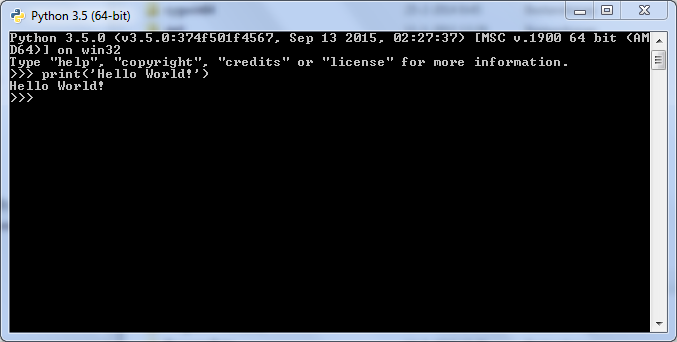
\includegraphics[scale=0.5]{Python35_(64-bit)}
	\caption{Python console met eerste commando}
	\label{Python35_(64-bit)}
\end{figure}

Python code kan opgeslagen worden in eenvoudige tekst bestanden met de extentie "\textsf{.py}". Om deze te schrijven is een goede text editor met syntax highlighting aan te raden. In Windows is \emph{notepad++} een goed, open source alternatief met syntax highlighting voor Python en een groot aantal andere talen ingebouwd. \emph{notepad++} kan worden gedownload vanop \url{https://notepad-plus-plus.org/download/}.

Omdat Python vanuit een commandline interface zal worden aangeroepen is het interessant om een deftige console te installeren. \emph{ConEmu} is een open source console emulator met gelijkenissen aan \emph{bash} in Linux. Deze is te downloaden vanaf \url{http://sourceforge.net/projects/conemu/files/latest/download}. Simpelweg downloaden, unzippen in een folder naar keuze en klaar.

 	\section{Scripts}
Omdat het telkens opnieuw invoeren van commando's achter elkaar niet zo praktisch is, is het interessant om een reeks commando's op te slaan in een script en dit uit te voeren. Open een teksteditor en typ \lstinline{print('Hello World!')} en sla het bestand op als \textsf{hello\_world.py}. Om het bestand uit te voeren open je een console, navigeer naar de locatie waar je het bestand hebt opgeslagen, typ \lstinline[language=bash]{python hello\_world.py} en druk op enter.

Python heeft een aantal interessanten ingebouwde variabele types. Open een nieuw bestand, typ onderstaande commando's en sla het op als \textsf{variables.py}.
\lstinputlisting{examples/variables.py}

Voor het script ditmaal uit met het commando \lstinline[language=bash]{python -i variables.py}. De \lstinline[language=bash]{-i} zorgt ervoor dat python na het uitvoeren van alle commando's in het script naar de interactieve console gaat. Alle reeds gedefinieerde variabelen zijn nu ook beschipkbaar in de console. Typ bijvoorbeeld:
\begin{lstlisting}
E[3]
\end{lstlisting}
of:
\begin{lstlisting}
A+B
\end{lstlisting}

Zoals te merken in het voorgaande voorbeeld is Python zeer flexibel met data types. Zo kunnen een \emph{Integer} en een \emph{Float} met elkaar opgeteld worden en kan een \emph{List} elementen met verschillende datatypes bevatten. Een zeer interessante data type is het \emph{Dictionary} of \emph{dict}. Hierin kunnen key / value paren worden opgeslagen en terug opgeroepen. Zowat elke Python variabele kan een \emph{Dictionary} key zijn wat dit type zeer flexibel maakt.

Het interessante aan elke programmeertaal is het maken van loops en voorwaarden: flow control. In python is dit zeer eenvoudig met behulp van \lstinline{for} lussen of \lstinline{if else} structuren:
\lstinputlisting{examples/flow_control.py}

In Python moet elk flow control element eindigen met een ":". De code binnen het element moet een tab inspringen. Dit zorgt voor een zekere leesbaarheid in de code. De \lstinline{range(10)} functie in de for lus maakt een \emph{List} met waarden van 0 tot en met 9. De \lstinline{.format(i)} functie formatteert zijn inhoud op de plaats van de accolade's in de voorafgaande string. De format functie is eigenlijk een methode van het \emph{String} datatype en geeft een hele reeks formatteer opties. Even zoeken op het net leert je heel veel over zulke ingebouwde functies.

Je kan over zowat elk datatype itereren. Een lus over een dictionary kan bijvoorbeeld op verschillende manieren. Ook itereren over verschillende variablen tegelijk is eenvoudig met de \lstinline{zip()} functie. Indien je itereert over een \emph{List} en de index van de variabelen wil gebruiken kan je de functie \lstinline{enumerate()} gebruiken:
\lstinputlisting{examples/flow_control_advanced.py}

Een set commando's die vaak op dezelfde manier gebruikt worden kan je groeperen in een functie. Een functie definieer je met het \lstinline{def} keywoord, gevolgd door de functie naam, de argument namen tussen haakjes en een dubbelpunt. Argumenten kunnen verplicht of optioneel zijn. voor optionele argumenten moet een default waarde opgegeven worden in de functie definitie. Alle verplichte argumenten moeten ook voor de optionle komen in de functie definitie. Wanneer een functie veel optionele argumenten heeft is het gemakkellijk om deze via naam-waarde paren op te geven, de volgorde is dan niet meer van belang:
\lstinputlisting{examples/functions.py}
Variabelen die binnen een functie gedefinieerd zijn bestaan ook enkel in de functie namespace. Bovenstaande code geeft dus een error omdat \lstinline{val} enkel in de functie namespace gedefinieerd is, niet in de globale namespace. Functies kunnen wel gebruik maken van variabelen in de globale namespace maar niet omgekeerd. Wanneer de bovenstaande code runt krijg je dan ook de volgende foutmelding:
\begin{lstlisting}
Traceback (most recent call last):
  File "C:\examples\functions.py", line 10, in <module>
    print(val)
NameError: name 'val' is not defined
\end{lstlisting}

	\section{Numpy en Matplotlib} 
Er bestaan enorm veel modules waarin specifieke functie gedefinieerd zijn voor gebruik in Python. Twee voor Ingenieurs interessante modules zijn \emph{Numpy}, een lineair algebra module en \emph{Matplotlib} een module voor het maken van wetenschappelijke figuren van hoge kwaliteit. Voor beide kunnen onofficiele windows installers worden gedownload via \url{http://www.lfd.uci.edu/~gohlke/pythonlibs/#numpy} en \url{http://www.lfd.uci.edu/~gohlke/pythonlibs/#matplotlib}. Gewoon de binary kiezen die overeenkomt met jou systeem architectuur, downloaden en installeren.


	\section{Object georiënteerd} 
	
 	\section{Modules}

\end{document}